\documentclass[11pt,a4paper]{article}

\usepackage{iftex}
\ifPDFTeX
  \usepackage[utf8]{inputenc}
  \usepackage[T1]{fontenc}
  \usepackage{lmodern}
\else
  \usepackage{fontspec}
\fi
\usepackage[spanish,es-tabla,es-noshorthands,es-nosectiondot]{babel}
\usepackage[margin=2.5cm]{geometry}
\usepackage{setspace}
\usepackage{graphicx}
\usepackage{booktabs}
\usepackage{tabularx}
\usepackage{array}
\usepackage{caption}
\usepackage{csquotes}
\usepackage{enumitem}
\usepackage[titles]{tocloft}
\usepackage[natbibapa]{apacite}
\usepackage{hyperref}
\usepackage{xurl}

\setstretch{1.12}
\setlist[itemize]{leftmargin=1.2em,itemsep=0.25em,topsep=0.35em}
\setlist[enumerate]{leftmargin=1.4em,itemsep=0.25em,topsep=0.35em}
\captionsetup{font=small,labelfont=bf,skip=0.5em,justification=raggedright,singlelinecheck=false,labelsep=period}
\setlength{\cftsecnumwidth}{2.8em}
\setlength{\cftsubsecnumwidth}{3.8em}
\renewcommand{\cftsecaftersnum}{.}
\renewcommand{\cftsubsecaftersnum}{.}
\renewcommand{\cftsecaftersnumb}{\ }
\renewcommand{\cftsubsecaftersnumb}{\ }
\makeatletter
\AtBeginDocument{%
  \renewcommand{\@seccntformat}[1]{\csname the#1\endcsname.\space}%
}
\makeatother
\babelhyphenation[spanish]{ob-ser-va-do pro-duc-tos}
\hypersetup{
  colorlinks=true,
  linkcolor=black,
  citecolor=black,
  urlcolor=black,
  pdftitle={NutriMatch. Trabajo final},
  pdfauthor={Paola Castañeda Covarrubias},
  pdflang={es}
}

\graphicspath{{figuras/}}

\newcommand{\corte}{2 de octubre de 2026}
\newcommand{\archivo}{\texttt{dataset\_referencia\_20261002}}

\title{NutriMatch:\\apoyo a la decisión de compra de alimentos empacados en México}
\author{Paola Castañeda Covarrubias}
\date{3 de octubre de 2026}

\begin{document}

\begin{titlepage}
  \centering
  \vspace*{2.2cm}
  {\large Diplomado en Ciencia de Datos\par}
  \vspace{1.6cm}
  {\LARGE\bfseries NutriMatch\par}
  \vspace{0.7cm}
  {\Large Apoyo a la decisión de compra\\de alimentos empacados en México\par}
  \vspace{1.4cm}
  {\large Trabajo final\par}
  \vspace{2.2cm}
  Paola Castañeda Covarrubias\par
  \vspace{0.4cm}
  3 de octubre de 2026\par
  \vfill
  \begin{minipage}{0.86\textwidth}
    \small\centering
    NutriMatch ayuda a comparar alimentos empacados con la información publicada y con lo que la persona declara.
    No emite diagnósticos ni dice que un alimento sea saludable para toda la población.
  \end{minipage}
  \vspace{1.2cm}
\end{titlepage}

\tableofcontents
\newpage

\section{Resumen}

Dos productos parecidos pueden verse iguales en el anaquel y traer datos distintos. Uno declara azúcar y fibra. Otro no dice nada de alérgenos. Otro no tiene precio. Compararlos a ojo mezcla lo que el producto afirma con lo que el registro simplemente no trae.

La pregunta es cómo convertir esa información, heterogénea e incompleta, en una comparación útil y repetible, sin inventar lo que los datos no traen. La persona indica qué quiere privilegiar, si sigue una dieta vegana o vegetariana y qué alérgenos necesita evitar. El orden usa solo la información disponible y muestra con qué datos se armó. No afirma que un producto sea mejor para toda la población.

El catálogo sale de Open Food Facts, una base pública de fichas de alimentos, en su corte de México. Si existe un precio observado, se toma de Open Prices o de Quién es Quién en los Precios. El análisis de esos datos fijó el diseño: no inventar lo que falta, comparar la nutrición entre productos parecidos, usar solo cinco nutrientes con una dirección clara, afinar el grado de procesamiento con el número de aditivos y dejar el precio fuera del orden. El cálculo es determinista: las mismas entradas dan siempre el mismo resultado. NutriMatch no utiliza aprendizaje supervisado porque el catálogo no contiene un target observado que permita entrenar y evaluar de manera científicamente válida un modelo de recomendación. Dicho de otra forma, no hay compras registradas que sirvan de respuesta correcta para entrenar un modelo.

El archivo de este trabajo es del \corte: 13\,093 productos de México y 273 columnas, sin códigos repetidos. De ellos, 5\,864 (44{,}79\,\%) tienen información suficiente para comparar nutrición y procesamiento antes de conocer a la persona. El precio real existe en 259 productos. Los otros 12\,834 no tienen precio. En un perfil de ejemplo, el orden reúne 113 productos, y 114 si cambian las prioridades.

Para revisar la parte nutricional se usó Nutri-Score como contraste externo, no como verdad del sistema. En 6\,035 productos, las dos medidas van en sentidos opuestos, que es lo esperado: la correlación de Spearman es $-0{,}475683$. Doce de trece casos revisados a mano coinciden. El caso restante difiere en el nombre, no en el puntaje.

La limitación principal es doble. Muchos registros no traen la información necesaria, y nadie observó la compra final. El sistema puede ordenar lo que está documentado. No puede decir si la persona elegirá el producto que quedó primero.

\section{Introducción}

Comprar un alimento empacado suele ofrecer varias presentaciones del mismo tipo. La etiqueta trae números, ingredientes y declaraciones, pero no todos los productos traen los mismos campos. Uno declara azúcar y fibra. Otro no trae el grado de procesamiento. Otro no dice nada sobre alérgenos, es decir, sobre sustancias que una persona necesita evitar. La decisión se toma con ese material, no con una ficha completa.

Comparar esos productos es difícil por tres razones que llegan juntas. Los datos no comparten la misma escala: un nutriente se expresa por 100\,g o 100\,mL, el procesamiento es un grupo, una etiqueta es un sí o un no, y el precio, cuando existe, es un monto. Además, la información no está igual de completa en todos los registros. Y lo que una persona quiere privilegiar puede no coincidir con lo que privilegia otra.

NutriMatch aborda esa comparación para alimentos empacados de México. Toma la información publicada y lo que la persona declara, y devuelve un orden que se puede explicar. Sirve para ver un producto, contrastarlo con otros parecidos y revisar qué dato sostuvo el resultado. La persona decide si se queda con él, si lo cambia o si lo deja fuera.

El sistema no prescribe una dieta, no interpreta síntomas y no observa la compra que ocurre después. Un resultado alto indica mayor compatibilidad con lo que la persona declaró y con la información disponible. No indica que el alimento sea adecuado para cualquier persona.

El documento sigue ese camino. Primero se precisa el problema y qué necesitaría la persona para usar una comparación así. Después se revisa si los datos publicados alcanzaban, qué mostró la exploración y qué decisiones salieron de esos hallazgos. Luego se explica cómo se prepararon los datos, cómo se convierten en un orden y cómo se comprobó que el sistema hace lo que se diseñó para hacer. El cierre vuelve al uso: qué queda resuelto, qué se puede defender y qué no.

Las cifras corresponden al archivo \archivo, del \corte. Si aparece el 19 de septiembre de 2026, es un corte anterior y se señala como histórico.

\section{Planteamiento del problema}

\subsection{El problema}

La decisión es concreta. Hay dos o más alimentos empacados parecidos, y hay que elegir. La dificultad es que la ficha de cada uno está incompleta de una manera distinta.

La información útil existe, pero está repartida. Llega como nutrientes por 100\,g o 100\,mL, como un grupo de procesamiento, como etiquetas, como alérgenos y trazas, como una lista de ingredientes y, en pocos casos, como un precio observado. Las trazas indican que el producto puede contener un alérgeno, aunque no sea un ingrediente principal. Cada dato responde una pregunta distinta. Ninguno, por sí solo, alcanza para ordenar la compra.

A eso se suma lo que no está. Un registro puede traer el nutriente y no la categoría que permitiría compararlo con productos parecidos. Puede traer el nombre y no decir nada sobre alérgenos. Puede no traer precio. Ese hueco no es un valor del alimento. Es la falta de una afirmación de la fuente.

Si ese silencio se lee como un hecho, la comparación se deforma. Leer \enquote{no hay dato de cacahuate} como \enquote{no contiene cacahuate} haría parecer apta a la mayor parte del catálogo, por falta de documentación y no por evidencia. Leer un precio ausente como cero haría parecer gratuitos a los productos sin precio. Contar un nutriente ausente como el valor más alto o el más bajo de la escala premiaría o castigaría el hueco.

De ahí sale un principio del proyecto. Un dato ausente no es un cero. Cero significa que la fuente afirmó un valor, por ejemplo que el producto no declara azúcar. Nulo significa que la fuente no trajo el dato. Si esa diferencia no se respeta, el orden parece completo y no lo es.

\subsection{Relevancia y alcance}

La compra ocurre con lo que está publicado, no con el dato que convendría tener. Por eso el problema importa: una comparación útil tiene que trabajar con fichas reales, incompletas y distintas entre sí. El proyecto se limita a alimentos empacados del corte mexicano usado por NutriMatch. No observa el anaquel del día, no registra compras y no describe a un grupo de personas.

La pregunta del trabajo es esta: ¿cómo convertir un catálogo heterogéneo de alimentos empacados en una comparación útil y reproducible para apoyar una decisión de compra, sin inventar información que los datos no contienen? Heterogéneo quiere decir que los datos son de tipos distintos y no llegan completos en todos los productos.

Esa pregunta, para quien compra, no es una fórmula. Es una decisión frente a varias opciones parecidas. La estrategia siguiente dice quién es esa persona, qué necesita y qué puede hacer con el resultado.

\section{Estrategia}

Quien está frente a varias opciones parecidas no necesita otra tabla de nutrientes. Necesita poder interpretar lo que sí hay y compararlo según lo que importa en esa compra. NutriMatch no decide por la persona ni dice cuál alimento es mejor en general. Ayuda a encontrar, entender y comparar opciones para tomar una decisión de compra con la información disponible y con las prioridades que ella declara.

\subsection{Usuarios objetivo}

La aplicación está pensada para quien compra alimentos empacados y, ante productos similares, quiere más elementos para elegir. Puede ser la compra de la semana, la búsqueda de un sustituto de algo que ya consume o simplemente una situación en la que dos opciones parecen iguales.

No hace falta saber de nutrición ni de Ciencia de Datos. Hace falta poder decir, de forma sencilla, qué importa más al elegir: la información nutricional, el nivel de procesamiento o ciertas características del producto. También se puede indicar si la alimentación es vegetariana o vegana y si hay que evitar algún alérgeno.

Esa persona no busca un diagnóstico ni una recomendación médica. Busca decidir la compra con lo que los datos permiten afirmar.

No se observó a compradores reales ni se midieron características como edad, ingreso o ciudad. El perfil que aparece en la evaluación es un ejemplo para observar qué ocurre cuando cambian las prioridades. No representa a una persona registrada.

\subsection{Necesidad}

La necesidad aparece cuando hay varias opciones parecidas y la información para compararlas está repartida en la etiqueta, o no está igual de completa en todos los productos. Revisar a mano nutrientes, sellos, ingredientes, restricciones y precio vuelve más difícil la comparación. Si además falta un dato, leer ese silencio como si la característica no existiera puede cambiar el sentido de la elección.

Lo que hace falta, entonces, es reunir la información disponible y presentarla de modo que la persona pueda pasar de tener varias opciones frente a ella a elegir entre ellas.

\subsection{Accionables}

El resultado no se queda en un número. Sirve para decidir qué hacer con el producto que se está mirando. La persona puede conservarlo, descartarlo, buscar una alternativa, sustituirlo o revisar con más cuidado alguna restricción.

En el carrito, el conjunto elegido también se puede observar mediante los grupos del Plato del Bien Comer: verduras y frutas, cereales, leguminosas y alimentos de origen animal, además de lo que no se puede clasificar \citep{nom0432013}. Esta vista da contexto a la compra y permite revisar el conjunto elegido. No es un diagnóstico.

\begin{table}[ht]
  \centering
  \caption{Acciones de compra que permite el resultado.}
  \label{tab:accionables}
  \small
  \begin{tabularx}{\textwidth}{>{\raggedright\arraybackslash}p{3.4cm}XX}
    \toprule
    Acción & Qué puede hacer la persona & Para qué le sirve \\
    \midrule
    Conservar un producto &
    Revisar el resultado y decidir si lo lleva. &
    Elegir con base en las prioridades que declaró. \\
    \addlinespace
    Descartarlo &
    Dejar fuera una opción que no corresponde a lo que busca o que no se puede verificar. &
    No quedarse con un producto solo porque se parece a los demás. \\
    \addlinespace
    Explorar alternativas &
    Consultar otros productos del mismo tipo. &
    Ver opciones comparables sin recorrer todo el catálogo. \\
    \addlinespace
    Sustituirlo &
    Cambiar el producto por otra opción de ese mismo tipo. &
    Ajustar la elección sin empezar la búsqueda de cero. \\
    \addlinespace
    Revisar restricciones &
    Consultar información sobre dieta y alérgenos. &
    Saber si el producto no cumple una condición o si no hay información suficiente para confirmarlo. \\
    \addlinespace
    Cerrar la compra &
    Llevar lo elegido al carrito y revisar el conjunto. &
    Pasar de la comparación de un producto a la decisión de compra. \\
    \bottomrule
  \end{tabularx}
\end{table}

Estos accionables conectan el resultado del sistema con una decisión concreta. NutriMatch no busca que la persona interprete un puntaje por sí solo, sino que pueda utilizar la comparación para decidir qué producto conservar, cuál descartar o por cuál sustituirlo.

\subsection{Propuesta de solución}

La comparación empieza con una pregunta sencilla: ¿qué es más importante en esta compra?

La persona ordena nutrición, procesamiento y las características que valora. A partir de ese orden se organizan los productos y se muestra cuáles se ajustan más a esas prioridades.

Se puede empezar por un producto concreto, ver sus características y después mirar alternativas del mismo tipo. No hace falta recorrer el catálogo entero para encontrar un sustituto.

El resultado se lee sin interpretar una fórmula. Se distingue si el producto entra en la comparación, si la información no alcanza o si una condición no se puede confirmar. El precio se muestra cuando existe una observación real. Si el monto es de demostración, se identifica como tal: informa la ficha y el recorrido de compra, pero no decide el orden.

En resumen, no se le dice a la persona qué debe comer. Se convierte información dispersa en una comparación que puede utilizar en el momento de comprar. La forma en que esa comparación se construye a partir de los datos se explica en las secciones siguientes.

\subsection{Usabilidad}

El recorrido sigue el orden de una compra: identificar un producto, entenderlo, comparar alternativas y decidir si se lleva.

No hace falta conocer el cálculo. Se busca un producto, se revisa su ficha, se consultan alternativas y se elige. Las tres prioridades se pueden ordenar según lo que pese más en esa compra.

Dieta y alérgenos se declaran dentro del mismo recorrido. La aplicación distingue entre una condición que sí se puede identificar y una que no se puede confirmar. Así, la falta de un dato no se interpreta por sí sola como señal de que el producto es apto.

La información llega por etapas. Primero se muestra el resultado, para facilitar la decisión; después, el detalle, si hace falta. Quien solo quiere elegir entre dos productos no tiene que leer toda la parte técnica para utilizar la aplicación.

La decisión tampoco termina en la ficha. Lo elegido pasa al carrito, donde se pueden revisar las alertas y observar cómo se reparte el conjunto.

Este recorrido está implementado y puede seguirse sin conocer la fórmula que genera el resultado. Sin embargo, no se realizó una prueba formal con compradores ni una medición de satisfacción. Por ello, el proyecto puede describir y demostrar el flujo de uso, pero no afirmar que su usabilidad haya sido validada con personas reales.

\section{Descripción de los datos}

La estrategia pide una comparación que se pueda usar en la compra y que no invente lo que falta. El siguiente paso fue ver si había datos para sostenerla. Hacía falta la ficha del producto, con lo que declara y con lo que no trae, y un precio solo cuando alguien lo hubiera observado. El catálogo se armó con tres fuentes públicas. Cada una cubre una parte distinta. Ninguna, por sí sola, resuelve la comparación.

\subsection{Fuentes}

Open Food Facts aporta la ficha: nombre, marca, nutrientes por 100\,g o 100\,mL, categorías, ingredientes, alérgenos, trazas, etiquetas, grupo NOVA y aditivos \citep{openfoodfacts2026}. Es una base pública y colaborativa. Sin esa ficha no habría qué comparar. De ella salen la nutrición, el procesamiento y las restricciones de alergia y dieta.

Open Prices aporta un precio en pesos cuando el código de barras coincide de forma exacta \citep{openprices2026}. Sirve para informar un costo que sí se observó. No se usa para inventar el precio de los productos que no aparecen ahí.

Quién es Quién en los Precios, de la Procuraduría Federal del Consumidor, no publica código de barras. Un precio de esa fuente solo entra si la coincidencia por texto fue revisada, comparando marca, producto y presentación \citep{profeco2026}. Se muestra como precio de referencia de una presentación parecida, y se indica cómo se hizo la coincidencia y qué tan confiable quedó.

\subsection{Integración}

Cada producto se identifica por su código de barras. No se juntaron presentaciones: el mismo nombre en otro tamaño o en otro sabor puede ser otro producto. Comparar solo por nombre habría mezclado productos distintos.

El archivo parte del export de Open Food Facts llamado \texttt{off\_csv\_20260929}. En el filtro de México, ese export tenía 16\,851 productos. Sobre ese punto de partida se aplicaron tres filtros. En este documento se llaman candados. Ese conteo de 16\,851 es el inicio de la construcción, no el catálogo que se evalúa aquí.

\begin{table}[ht]
  \centering
  \caption{Candados que producen el catálogo operativo. Fuente: metadato de \archivo.}
  \label{tab:candados}
  \begin{tabular}{lrr}
    \toprule
    Paso & Productos & Salen \\
    \midrule
    Filtro de México en el export & 16\,851 & \\
    Producto no alimentario & 16\,848 & 3 \\
    Integridad de identidad y nutrición & 13\,111 & 3\,737 \\
    Identidad del nombre & 13\,093 & 18 \\
    \bottomrule
  \end{tabular}
\end{table}

El primer filtro retira tres productos que no son alimentos. El segundo pide que la identidad y la nutrición del registro se sostengan, y es el que más reduce el archivo. El tercero retira 18 registros cuyo nombre no queda identificado. El resultado, 13\,093 productos y 273 columnas, es el catálogo operativo de este trabajo. No es todavía el conjunto que se puede ordenar: eso depende de la cobertura, y se mide en la exploración. Para comprobar que los cálculos usan este archivo y no otro, se calculó su huella SHA-256:

\begin{center}
\small\texttt{a621d471a2f47aa09ba481408d95a7a808fe84bd2fa7205c56fa050e1c66045b}
\end{center}

\noindent Hay cero códigos duplicados. El cuaderno de trabajo comprueba esa huella antes de continuar. Las dos fuentes de precio no comparten códigos. Si un código tiene varias observaciones, se conserva la real más reciente.

\subsection{Estructura}

Cada fila es un producto. Las columnas que vienen del export son observaciones de Open Food Facts. Lo que NutriMatch calcula o recupera después lleva un estado: real, si se observó; derivado, si se calculó a partir de datos reales; o no disponible, si se sabe que no hay dato. El estado imputado, que significaría un valor estimado para rellenar un hueco, existe como nombre en el proyecto y no se usa en este catálogo. El estado sintético tampoco se escribe en el archivo. Aparece solo en la ficha, cuando no hay precio observado, y la pantalla lo llama precio de demostración.

El nombre que se muestra se busca en este orden: nombre del producto, nombre genérico y nombre abreviado. El texto \enquote{Cargando…} se trata como vacío. En este corte, 12\,712 productos tienen nombre visible y 11\,606 tienen marca. Si ninguno de esos campos tiene dato, el nombre queda vacío. No se inventa un título.

\subsection{Calidad}

La calidad de información resume siete piezas de disponibilidad y consistencia: nutrición, ingredientes, categoría, NOVA, aditivos, etiquetas y coherencia física. Dice qué tan documentado está el registro. No mide compatibilidad con un perfil y no entra al orden.

\begin{table}[ht]
  \centering
  \caption{Calidad de información del catálogo operativo. Fuente: notebook maestro, corte del \corte.}
  \label{tab:calidad}
  \begin{tabular}{lr}
    \toprule
    Nivel & Productos \\
    \midrule
    Alta & 6\,102 \\
    Media & 1\,511 \\
    Baja & 1\,274 \\
    Insuficiente & 4\,206 \\
    \bottomrule
  \end{tabular}
\end{table}

En el perfil de ejemplo, los 4\,206 registros de calidad insuficiente caen en la banda de información no verificable, no en el orden. Tener calidad alta tampoco garantiza entrar: en ese mismo perfil, 3\,360 productos de calidad alta quedan fuera por alergia o dieta. La calidad describe el registro. La banda describe la decisión.

\subsection{Relevancia y límites}

El catálogo sirve porque cubre el tipo de producto que la persona compara y porque conserva los huecos en lugar de disimularlos. También tiene límites medidos. Alérgenos, trazas, etiquetas y precio cubren poco. El precio real existe para 259 productos: 239 de Open Prices y 20 de PROFECO. Los otros 12\,834 no tienen precio. No hay un precio igual a cero.

Open Food Facts se actualiza, así que un corte posterior puede cambiar los conteos. Por eso cada resultado de este documento queda atado a la huella del archivo. Con el catálogo ya delimitado, el análisis siguiente pregunta qué se puede afirmar con esos datos y qué decisiones se siguen de ellos.

\section{Análisis exploratorio de datos}

El catálogo operativo ya está cerrado. La exploración pregunta si la información que la compra necesita está realmente ahí, y qué decisión se sigue de lo que se encuentra. Se usó el archivo oficial y las mismas funciones que usa la aplicación. Cada hallazgo deja una pieza del orden. No es una colección de gráficas sueltas.

\subsection{Cuánta información hay}

La primera pregunta fue cuántos productos se pueden comparar de verdad.

De 13\,093 productos, 7\,568 tienen una categoría de referencia (57{,}80\,\%), esto es, un grupo de productos parecidos contra el cual comparar. 6\,998 tienen al menos cuatro percentiles del núcleo (53{,}45\,\%). Un percentil es el puesto de un nutriente dentro de su categoría, en una escala de 0 a 100. 6\,780 tienen procesamiento calculable (51{,}78\,\%). El universo puntuable junta procesamiento y al menos cuatro de esos percentiles: 5\,864 productos, el 44{,}79\,\% del catálogo. Son productos con los que se puede armar la comparación antes de conocer a la persona. No son productos recomendados. La categoría de referencia no entra en esa regla: es la condición propia de la nutrición. La figura~\ref{fig:disponibilidad} muestra el contraste. Nutrición y procesamiento llegan a cerca de la mitad del catálogo. Etiquetas, alérgenos, trazas y precio cubren mucho menos.

\begin{figure}[ht]
  \centering
  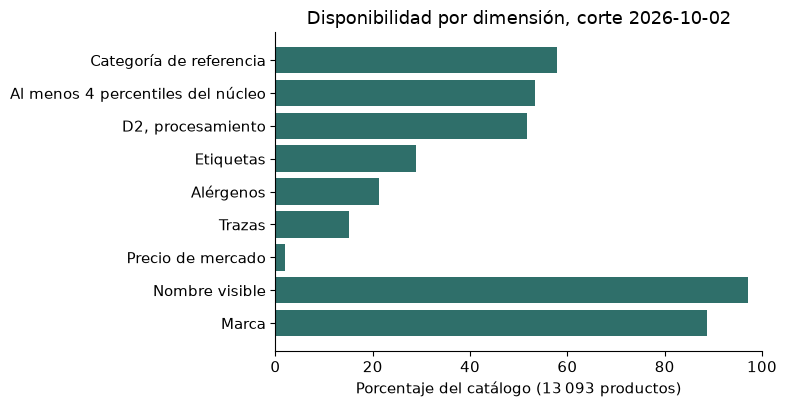
\includegraphics[width=0.92\textwidth]{disponibilidad.png}
  \caption{Productos con dato en cada bloque del catálogo. Fuente: notebook maestro, corte del \corte.}
  \label{fig:disponibilidad}
\end{figure}

De ahí salen tres conjuntos que no se deben mezclar. El catálogo operativo tiene 13\,093 productos. El universo puntuable tiene 5\,864. El orden de una persona es otro conjunto, más chico, y solo aparece cuando ya hay un perfil. Estar en el catálogo no basta para comparar. Estar en el universo puntuable no basta para aparecer en el orden de alguien.

En un corte anterior, del 19 de septiembre de 2026, otra regla más estricta sobre 16\,851 productos dejaba 5\,856 (34{,}8\,\%) en una versión temprana de ese universo. Describe otro archivo. No se usa en las decisiones de este documento.

\subsection{Faltantes}

La cobertura no es pareja. La pregunta siguiente es si esos huecos se pueden reconstruir.

Los huecos de la nutrición, de la categoría y de variables cercanas se concentran en registros que tampoco traen ingredientes, o que Open Food Facts ya marca como incompletos. No aparecen como un valor que se pueda copiar de productos parecidos. Falta información porque el registro está poco documentado, no porque el nutriente valga cero.

Por eso un faltante se guarda como nulo y se marca, para saber que el dato no vino. No se imputan nutrientes, alérgenos, etiquetas, dieta, grupo NOVA ni precio. Imputar sería rellenar el hueco con un estimado. En el orden, una parte sin dato no entra al promedio como cero. Si lo disponible pesa menos de la mitad de lo que la persona pidió, el producto sale de la comparación. Inventar el dato cambiaría el sentido del resultado y, en alergias, el riesgo.

\subsection{Nutrición}

Entre los productos que sí traen nutrientes, no todos sirven para ordenar. Azúcar, sal y grasa saturada tienen una dirección clara dentro de esta comparación: menos es mejor. Fibra y proteína, al revés: más es mejor. Esa dirección solo ordena esta parte del cálculo. No dice que el alimento convenga a cualquier persona.

Energía, grasa total y carbohidratos también tienen percentil y se muestran en la ficha. No hay una meta única que diga si conviene que suban o que bajen para toda la población, así que no se suman. La figura~\ref{fig:nutrientes} muestra la distribución de los cinco que sí entran. La señal nutricional resume esos cinco, no toda la etiqueta.

\begin{figure}[ht]
  \centering
  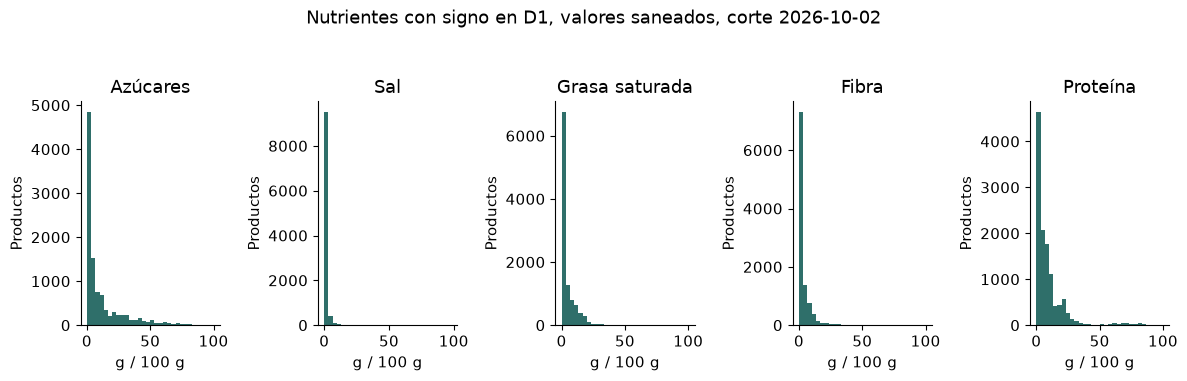
\includegraphics[width=\textwidth]{nutrientes_d1.png}
  \caption{Distribución de los cinco nutrientes que entran a la dimensión nutricional, en escala de percentil. Fuente: notebook maestro, corte del \corte.}
  \label{fig:nutrientes}
\end{figure}

\subsection{Categorías}

Un nutriente con dirección clara todavía necesita un grupo. Comparar un yogur con todo el catálogo mezclaría alimentos que no compiten en la misma decisión.

Open Food Facts ordena las categorías de lo general a lo específico, por ejemplo de lácteos a un tipo concreto de yogur. Se recorre esa lista desde lo más específico y se para en la primera etiqueta que aparece en al menos 30 productos. En este corte hay 201 categorías de referencia, y ninguna de esas etiquetas está por debajo de 30. Aun así, el grupo con el que se compara un producto puede ser menor, porque no todos los que mencionan la etiqueta la reciben como categoría elegida. La mediana de ese grupo es 27 productos. Hay 5\,525 productos sin categoría de referencia. La figura~\ref{fig:categorias} separa cuántas veces aparece la etiqueta y cuántos productos quedan en el grupo.

\begin{figure}[ht]
  \centering
  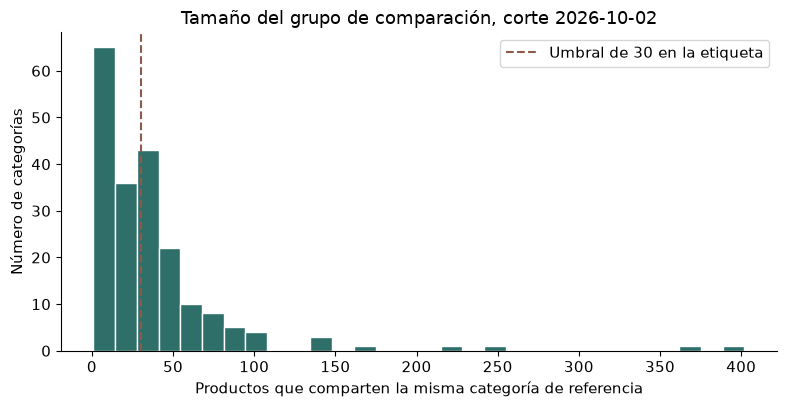
\includegraphics[width=0.92\textwidth]{categorias.png}
  \caption{Tamaño del grupo con el que se compara cada producto. Fuente: notebook maestro, corte del \corte.}
  \label{fig:categorias}
\end{figure}

Si ninguna categoría alcanza el mínimo, la nutrición queda sin dato para ese producto. No se compara contra todo el catálogo. El percentil se calcula dentro de la categoría elegida. Sin categoría, la nutrición no aporta al orden.

\subsection{Procesamiento}

La nutrición no agota la comparación. La segunda pieza que la persona puede privilegiar es el grado de procesamiento. NOVA clasifica los alimentos en cuatro grupos, del menos procesado al ultraprocesado \citep{monteiro2018nova}. Aquí esa clasificación ordena una escala. No afirma que un alimento sea adecuado para cualquier persona.

La pregunta era si el grupo, por sí solo, distingue productos en este catálogo. De los que sí tienen grupo, la mayoría está en el 4: 4\,709, frente a 804 en el grupo 1, 189 en el grupo 2 y 1\,078 en el grupo 3. Hay 6\,313 productos sin grupo. Con tanta concentración en un solo grupo, NOVA solo no separa la compra. El número de aditivos, los ingredientes añadidos que el registro enumera, se mueve en el mismo sentido que el grupo y cubre un poco más de productos. La figura~\ref{fig:nova} muestra esa concentración.

\begin{figure}[ht]
  \centering
  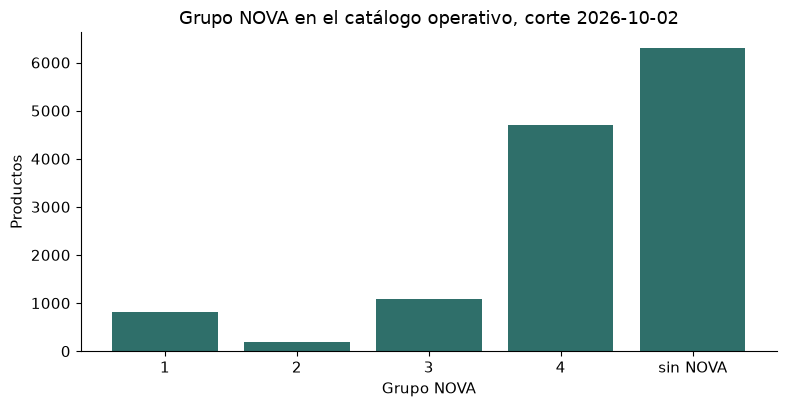
\includegraphics[width=0.78\textwidth]{nova.png}
  \caption{Productos por grupo NOVA. Fuente: notebook maestro, corte del \corte.}
  \label{fig:nova}
\end{figure}

El grupo fija un tramo de la escala. Los aditivos mueven al producto dentro de ese tramo, para no dejar juntos a miles de productos del grupo 4. Si no hay grupo, esta parte queda nula: no se inventa un NOVA. Los aditivos no forman una cuarta señal. Solo ajustan el tramo que el grupo ya fijó.

\subsection{Preferencias}

Nutrición y procesamiento se pueden calcular antes de conocer a la persona. Las etiquetas no. Solo tienen sentido frente a lo que esa persona dice que valora.

Solo 3\,776 productos tienen etiquetas. En el perfil de ejemplo, que valora orgánico y sin gluten, 9\,317 productos no tienen con qué comparar y 3\,068 tienen etiquetas, pero ninguna de las dos. Solo 708 presentan al menos una. Si el producto no tiene etiquetas, o si la persona no declaró ninguna, esta parte queda nula. Vale cero solo cuando hay etiquetas y ninguna coincide. No se rellena la preferencia. El cálculo espera al perfil.

\subsection{Precio y calidad}

El precio y la calidad del registro se ven con facilidad, y resulta tentador usarlos para desempatar. Los datos no sostienen ese uso.

El precio de mercado existe en 259 productos (figura~\ref{fig:precios}). Es poco frente al catálogo, así que un orden por precio dejaría fuera a casi todos. La calidad de información, en la figura~\ref{fig:calidad}, describe si el registro está documentado. No mide si el producto encaja con un perfil. Las dos se muestran. No entran al puntaje ni a los filtros del orden. Un precio ausente no se sustituye, dentro del catálogo, por una estimación de mercado.

\begin{figure}[ht]
  \centering
  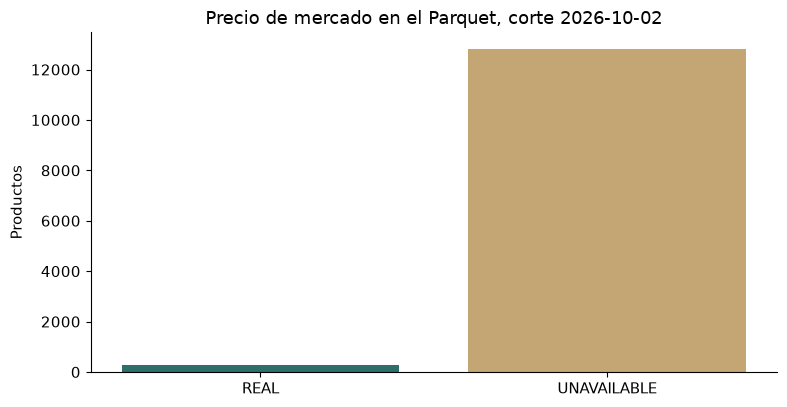
\includegraphics[width=0.72\textwidth]{precios.png}
  \caption{Precio observado y precio ausente. Fuente: notebook maestro, corte del \corte.}
  \label{fig:precios}
\end{figure}

\begin{figure}[ht]
  \centering
  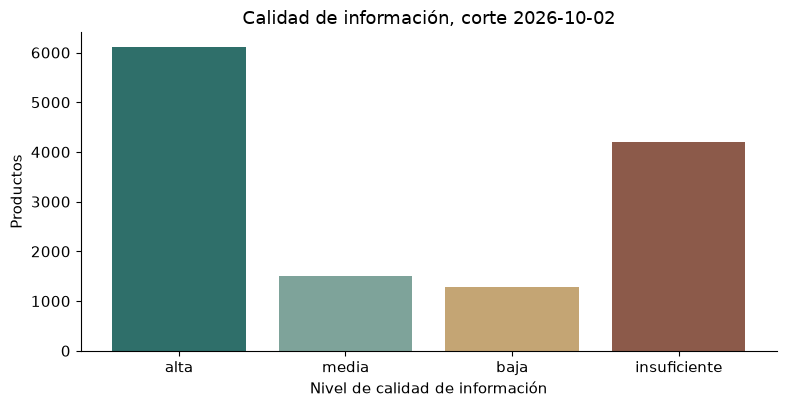
\includegraphics[width=0.72\textwidth]{calidad.png}
  \caption{Calidad de información del registro. Fuente: notebook maestro, corte del \corte.}
  \label{fig:calidad}
\end{figure}

Cada hallazgo dejó una decisión. La cobertura desigual separa catálogo, universo puntuable y orden de un perfil. Los faltantes se conservan como nulos. La nutrición usa cinco nutrientes y se calcula dentro de la categoría. El procesamiento toma el grupo NOVA y lo ajusta con aditivos, sin inventar el grupo cuando falta. Las etiquetas esperan al perfil. El precio y la calidad se muestran y no ordenan. La preparación de los datos tiene que respetar esas decisiones, no volver a discutirlas.

\section{Procesamiento de datos}

La exploración mostró que los faltantes son frecuentes y que siguen qué tan documentado está el registro. Esta etapa no vuelve a ese hallazgo: lo prepara para el cálculo. Un dato ausente no es un cero. Cero significa que la fuente afirmó un valor, por ejemplo que el producto no declara azúcar. Nulo significa que la fuente no trajo el dato. Las transformaciones siguientes evitan que esas dos situaciones se confundan.

\subsection{Limpieza}

El código de barras se guarda como texto, para no perder un cero inicial. Si se leyera como número, un código que empieza con cero podría cambiar. Un texto ausente que llega como un valor numérico vacío se trata como ausencia antes de separar etiquetas o de decidir si una parte del cálculo tiene dato. El texto \enquote{Cargando…} no se acepta como nombre.

Los valores fuera de un rango físico plausible se marcan como extremos. Ese producto deja de aportar al percentil y a las estadísticas de su categoría en esa medida. El valor original sigue visible en la ficha. Ocultarlo sería reescribir el registro. En este corte hay 56 registros con sal fuera de rango. En 55, la relación entre la sal y el sodio del mismo producto es aproximadamente 2{,}5, y el valor dividido entre 1\,000 cae en un rango válido. Esos 55 se corrigen con los dos campos del propio producto, y la corrección queda marcada. El caso típico es una sal anotada mil veces más alta, como si la unidad se hubiera corrido. El registro que no cumple esa relación permanece fuera de rango, sin corrección. Hay además 57 registros en los que la suma de macronutrientes supera 100. Esa marca es informativa y no borra los nutrientes.

\subsection{Valores faltantes e imputación}

No se imputan precio, alérgenos, etiquetas, dieta, grupo NOVA ni los nutrientes del núcleo. Imputar sería poner un valor estimado donde la fuente no dijo nada. El catálogo no contiene valores de ese tipo. Cada ausente queda nulo, con una bandera que dice que el dato no está, para que el cálculo sepa qué parte puede usar.

Tampoco se crearon productos artificiales para agrandar el catálogo. Un registro inventado no es una observación. El precio de demostración que a veces aparece en la ficha es otra cosa: un entero entre 12 y 180 pesos, siempre el mismo para el mismo código, marcado como simulado. No se escribe en el archivo y el orden no lo usa. Sirve para recorrer la pantalla, no para completar los datos.

\subsection{Otras transformaciones}

La categoría de referencia, los percentiles y la parte de procesamiento se calculan una vez y quedan en el archivo. No dependen de lo que la persona declare. Las etiquetas y el resultado final se calculan cuando llega el perfil. Por eso, repetir una corrida exige el mismo archivo, el mismo perfil y el mismo conjunto de productos.

Con lo observado, lo corregido y lo ausente ya separados, el paso siguiente es convertirlos en las piezas que el orden combina.

\section{Ingeniería de variables}

Las variables de esta sección resuelven problemas que la exploración ya dejó planteados. Se calculan a partir de datos observados. No predicen un valor que la fuente no trajo. La tabla~\ref{tab:variables} resume el papel de cada una. El detalle, y la razón de cada transformación, va después.

\begin{table}[ht]
  \centering
  \caption{Variables derivadas y papel en la decisión.}
  \label{tab:variables}
  \small
  \begin{tabularx}{\textwidth}{lX}
    \toprule
    Variable & Papel \\
    \midrule
    Categoría de referencia & Define el grupo de comparación. Si no hay una etiqueta con al menos 30 productos, no hay dimensión nutricional. \\
    Percentiles & Sitúan cada nutriente dentro de su categoría, en escala de 0 a 100. Un percentil exige al menos cinco productos con dato saneado. \\
    Dimensión nutricional & Promedio de los percentiles con dirección: azúcar, sal y grasa saturada se invierten; fibra y proteína se usan tal cual. Se calcula al cargar el catálogo. \\
    Dimensión de procesamiento & Banda del grupo NOVA, afinada con aditivos. Ya está en el archivo. \\
    Dimensión de etiquetas & Porcentaje de las etiquetas valoradas que el producto presenta. Se calcula con el perfil. \\
    Cobertura & Peso de las dimensiones con dato, dividido entre el peso del perfil. \\
    Resultado final & Promedio ponderado de las dimensiones disponibles. Nulo si la cobertura es menor que 0{,}5. \\
    Universo puntuable & Procesamiento presente y al menos cuatro de ocho percentiles. Es previo al perfil. \\
    Calidad y precio & Se muestran. No entran al resultado. \\
    \bottomrule
  \end{tabularx}
\end{table}

\subsection{Percentiles y dimensión nutricional}

Azúcar y fibra no se miden en la misma escala, y dentro de una categoría sus distribuciones tampoco son iguales. Para compararlas entre productos parecidos se usó el puesto de cada uno frente a los demás de su categoría. Ese puesto es el percentil. No es una fracción entre cero y uno. En este corte, el máximo observado es 100. Para calcular el percentil de un nutriente hacen falta al menos cinco productos con dato saneado en esa categoría. Si hay menos, ese percentil queda nulo.

La señal nutricional no promedia los ocho nutrientes del núcleo. Usa cinco, y solo los que tienen percentil. Si \(p\) es ese puesto, fibra y proteína aportan \(p\). Azúcar, sal y grasa saturada aportan \(100 - p\): en esos tres, un puesto alto significa más cantidad, y la señal los lee al revés. El resultado de esta parte es el promedio de los aportes que sí existen. Energía, grasa total y carbohidratos se quedan en la ficha.

Al cargar el catálogo, 7\,028 productos tienen esta señal calculable (53{,}68\,\%). El archivo en disco sigue teniendo 273 columnas. La señal se agrega en memoria y no se reescribe en el archivo.

\subsection{Procesamiento}

Cada grupo NOVA ocupa un tramo de 25 puntos: el grupo 1 entre 75 y 100, el 2 entre 50 y 75, el 3 entre 25 y 50, y el 4 entre 0 y 25 \citep{monteiro2018nova}. El techo del grupo \(g\) es \(100 - (g - 1) \times 25\). Dentro del tramo, los aditivos restan desde ese techo hacia abajo, hasta el percentil 95 de aditivos observado en los productos del grupo 4 de este mismo corte. Si el número de aditivos falta, se restan 12{,}5 puntos, la mitad del tramo, y el producto queda en el centro. Sin grupo, la señal es nula. Que falten los aditivos no se lee como si el producto tuviera cero aditivos.

\subsection{Etiquetas, cobertura y resultado}

La señal de etiquetas es el porcentaje de las etiquetas valoradas por la persona que el producto presenta. Queda nula si el producto no tiene etiquetas o si la persona no declaró ninguna. Es cero solo cuando hay etiquetas y ninguna coincide.

La persona ordena tres prioridades. Ese orden se convierte en pesos que suman 1: \(3/6\) (0{,}50) para la primera, \(2/6\) (0{,}33) para la segunda y \(1/6\) (0{,}17) para la tercera. No hay controles numéricos sueltos. La primera prioridad pesa la mitad. La segunda, cerca de un tercio. La tercera, el resto.

Si \(A\) son las partes con dato y \(w_d\) es el peso de cada una, la cobertura es la fracción del perfil que sí se pudo calcular:
\[
c = \frac{\sum_{d \in A} w_d}{w_1 + w_2 + w_3}.
\]
El resultado usa solo esas partes. Es su promedio ponderado:
\[
r = \frac{\sum_{d \in A} w_d \, s_d}{\sum_{d \in A} w_d},
\]
siempre que \(c \ge 0{,}5\). Si \(c < 0{,}5\), \(r\) queda nulo. La parte ausente no se sustituye por cero. Por eso el denominador es el peso de lo disponible, no el peso total.

Con estos pesos, cualquier par de partes suma al menos 0{,}5. Perder una sola no basta para salir del orden. El resultado queda nulo solo cuando la cobertura es menor que 0{,}5.

\subsection{Universo puntuable}

El universo puntuable se define antes de conocer a la persona. Pide procesamiento calculable y al menos cuatro de los ocho percentiles del núcleo. En este corte son 5\,864 productos, y la regla coincide con la bandera en todos los casos. La figura~\ref{fig:universo} muestra cómo se reduce el catálogo antes de aplicar un perfil.

Un producto puede estar en ese universo y, aun así, quedar fuera del orden de una persona, por alergia, por dieta o por cobertura. También puede entrar al orden sin estar en el universo, si las partes que ese perfil sí puede calcular pesan al menos la mitad. El cuarto producto del ejemplo de la sección~\ref{sec:evaluacion} es ese caso.

\begin{figure}[ht]
  \centering
  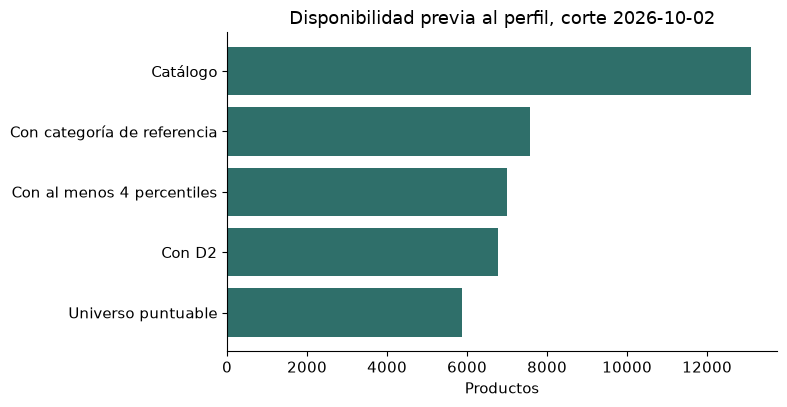
\includegraphics[width=0.92\textwidth]{universo.png}
  \caption{Estrechamiento del catálogo antes de aplicar un perfil. Fuente: notebook maestro, corte del \corte.}
  \label{fig:universo}
\end{figure}

Estas variables ya responden a lo que el análisis mostró. Falta la regla que las convierte, junto con el perfil, en un orden.

\section{Modelación y motor de decisión}

\subsection{De las variables a un orden}

Las variables ya dicen con quién se compara un producto, cómo se lee cada nutriente y qué hacer cuando falta un dato. Faltaba una forma repetible de pasar de esas variables, y de las prioridades de la persona, a un orden. Esa forma es una regla fija de compatibilidad. Aquí se llama motor. Las mismas entradas producen el mismo resultado y el mismo orden. No hay azar ni un ajuste entrenado con ejemplos.

La entrada es el catálogo y un perfil: el orden de tres prioridades, la dieta vegana o vegetariana si se declaró, los alérgenos a evitar y las etiquetas valoradas. Los pesos son los de la sección anterior: \(3/6\) (0{,}50), \(2/6\) (0{,}33) y \(1/6\) (0{,}17). La nutrición y el procesamiento llegan ya calculados. Las etiquetas y el resultado se arman cuando llega el perfil.

\subsection{Por qué no hay aprendizaje supervisado}

NutriMatch no utiliza aprendizaje supervisado en el MVP porque el catálogo no contiene un target observado que permita entrenar y evaluar de manera científicamente válida un modelo de recomendación. Un modelo supervisado aprende de ejemplos que ya traen la respuesta correcta. Aquí esa respuesta no existe: no hay historial de compra, no hay clics, no hay favoritos y no hay conversiones. El resultado, las tres señales y las bandas los calcula el propio sistema. Entrenar un modelo para predecirlos sería circular. La respuesta saldría de la misma regla que se quiere evaluar, y la prueba no diría nada nuevo.

Por eso el motor no es un modelo de aprendizaje automático. Es una regla de compatibilidad y de orden, a partir de lo que la persona declaró y de lo que el producto tiene observado. La falta de una respuesta de compra no se toma como una debilidad del sistema. Es la condición del problema: lo que se apoya es una comparación, no la predicción de una compra.

Tampoco se construyó un agrupamiento no supervisado. Ese tipo de análisis junta productos parecidos sin una respuesta previa. Podría describir el catálogo, pero no es lo que hoy ordena la compra. Hacerlo solo para nombrar una técnica no respondería la pregunta del proyecto. El orden sale de la regla que sigue.

\subsection{Alergias, dieta y bandas}

Alergias y dieta tienen tres estados: apto, no apto y no verificable. La alergia usa lo que el registro declara y las trazas, el aviso de que el producto puede contener el alérgeno. La dieta usa el análisis de ingredientes. Si los ingredientes no alcanzan para afirmar la dieta, el estado es no verificable. Decir que sí cumple, sin evidencia, inventaría un hecho.

El resultado combina las señales disponibles y las promedia según el peso de lo que sí tiene dato. Cada producto cae en una sola banda, en este orden:

\begin{enumerate}
  \item excluido, si la alergia no es apta o la dieta es incompatible; se cuenta y no se lista;
  \item no verificable, si la alergia o la dieta no se pueden afirmar;
  \item información insuficiente, si la cobertura es menor que 0{,}5;
  \item ranking, el resto, de mayor a menor resultado.
\end{enumerate}

El orden de las bandas importa. Un producto excluido no pasa a la banda de no verificable, y uno no verificable no se mezcla con los aptos. La búsqueda por nombre o por código ocurre antes de puntuar, sobre todo el catálogo.

\subsection{Salida}

La salida es un orden con el resultado, las tres señales, la banda, la cobertura y el estado de los datos. Las alternativas de un producto se buscan en su misma categoría, el grupo con el que ya se comparó la nutrición. El precio y Nutri-Score pueden acompañar la ficha. No cambian el orden de la lista.

Evaluar esta regla no es preguntar si predice una compra. Es preguntar si, con los mismos datos y el mismo perfil, hace lo que se diseñó para hacer. Eso corresponde a la sección siguiente.

\section{Evaluación}
\label{sec:evaluacion}

La evaluación pregunta si el motor hace lo que se diseñó para hacer. No pregunta si adivina una compra que nadie observó. Todas las cifras de esta sección salen del archivo del \corte, salvo cuando el texto dice que un resultado es histórico.

Hay cuatro comprobaciones. La primera revisa la regla del universo puntuable. La segunda contrasta trece productos revisados a mano. La tercera pregunta si la parte nutricional se mueve en un sentido razonable frente a una medida externa. La cuarta observa si el orden cambia cuando cambian las prioridades. Después se comprueba que el resultado no depende del azar, y se dice con claridad qué no queda demostrado.

\subsection{¿Se cumple la regla del universo puntuable?}

La regla se cumple sin diferencias: 5\,864 productos tienen procesamiento y al menos cuatro de ocho percentiles. La tabla~\ref{tab:cobertura} separa otros conteos que a veces se confunden con esa regla. Tener la señal nutricional, por ejemplo, no es lo mismo que pertenecer al universo puntuable.

\begin{table}[ht]
  \centering
  \caption{Cobertura del catálogo, antes de aplicar un perfil. Corte del \corte.}
  \label{tab:cobertura}
  \begin{tabular}{lrr}
    \toprule
    Condición & Productos & Porcentaje \\
    \midrule
    Categoría de referencia & 7\,568 & 57{,}80 \\
    Al menos un percentil del núcleo & 7\,047 & 53{,}82 \\
    Dimensión nutricional calculable & 7\,028 & 53{,}68 \\
    Al menos cuatro percentiles & 6\,998 & 53{,}45 \\
    Los ocho percentiles & 6\,083 & 46{,}46 \\
    Procesamiento disponible & 6\,780 & 51{,}78 \\
    Universo puntuable & 5\,864 & 44{,}79 \\
    \bottomrule
  \end{tabular}
\end{table}

\subsection{¿Los casos revisados producen el comportamiento esperado?}

Trece productos reales del catálogo se revisaron a mano, con el resultado esperado de cada caso. Sobre el archivo de este trabajo, doce coinciden. El caso \texttt{5060323907641} difiere solo en el nombre: la revisión esperaba el campo original, y el catálogo ya muestra el nombre tomado del nombre genérico, con el campo original vacío. El puntaje de ese producto sí se calcula. No falla ninguna de las tres señales. El caso no se quitó ni se reescribió para que la cuenta quedara en trece de trece.

\subsection{¿La dimensión nutricional se relaciona con un contraste externo?}

Nutri-Score es una etiqueta nutricional usada como contraste externo. No es la respuesta correcta del motor ni la meta del orden \citep{julia2017nutriscore}. En 6\,035 productos que tienen las dos medidas, la correlación de Spearman entre la señal nutricional y \texttt{nutriscore\_score} es $-0{,}475683$. Spearman resume si dos ordenamientos van en el mismo sentido o en sentidos opuestos.

El signo negativo es el que corresponde. En esta comparación, un valor alto indica mayor compatibilidad con las prioridades nutricionales declaradas. En Nutri-Score, la letra A es el extremo más favorable de esa escala y la E el menos favorable; el puntaje numérico, en cambio, es peor cuando sube. Una relación negativa es coherente con esas dos direcciones. No convierte a Nutri-Score en la verdad del sistema. El proyecto pidió, como mínimo de sanidad, una correlación menor o igual a $-0{,}3$. La cifra medida supera ese umbral en magnitud.

El promedio de la señal nutricional baja de la letra A a la letra E: 59{,}68, 54{,}80, 50{,}87, 49{,}00 y 41{,}57 (figura~\ref{fig:nutriscore}). Esa bajada comprueba la misma dirección.

\begin{figure}[ht]
  \centering
  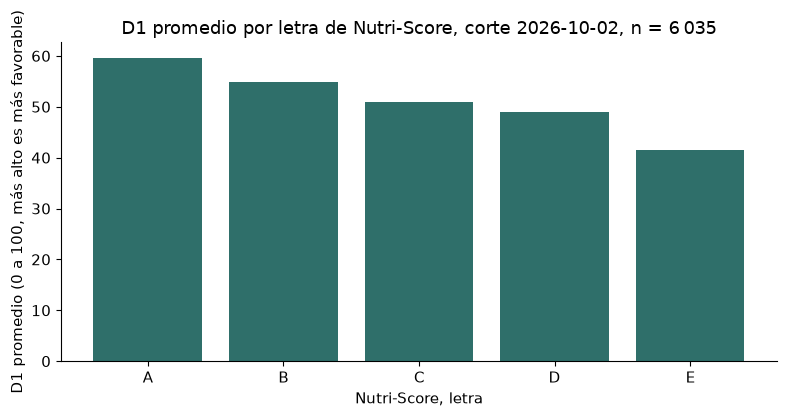
\includegraphics[width=0.86\textwidth]{d1_nutriscore.png}
  \caption{Dimensión nutricional promedio según la letra de Nutri-Score. \(n = 6\,035\). El título interno de la gráfica llama D1 a esa dimensión. Fuente: notebook maestro, corte del \corte.}
  \label{fig:nutriscore}
\end{figure}

El mismo contraste, calculado el 19 de septiembre de 2026 sobre otro archivo, dio \(n = 6\,041\) y una correlación de $-0{,}4747$. Es un resultado histórico. No sustituye la cifra de este corte.

\subsection{¿El resultado cambia cuando cambian las prioridades?}

El perfil de ejemplo evita gluten, declara dieta vegana, valora las etiquetas orgánico y sin gluten, y pone la nutrición en primer lugar, las etiquetas en segundo y el procesamiento en tercero. No es una persona observada. Con la regla de bandas de la aplicación, el catálogo queda así: 3\,808 excluidos, 9\,171 no verificables, 1 con información insuficiente y 113 en la banda de ranking. Si el procesamiento pasa al primer lugar y la nutrición al tercero, el orden tiene 114 productos. Los excluidos y los no verificables no cambian, porque no dependen de los pesos.

\begin{figure}[ht]
  \centering
  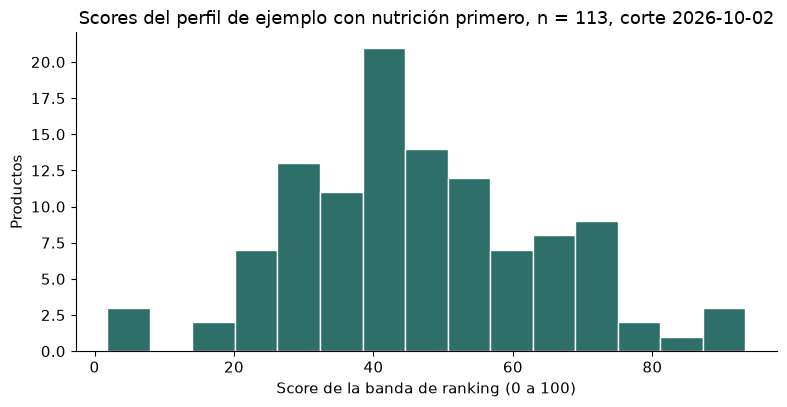
\includegraphics[width=0.86\textwidth]{scores_perfil.png}
  \caption{Resultados del orden cuando la nutrición es la primera prioridad. \(n = 113\). Fuente: notebook maestro, corte del \corte.}
  \label{fig:scores}
\end{figure}

Dentro de los 113, el primer producto obtiene 93{,}30. El cuarto, con resultado 83{,}33, no pertenece al universo puntuable: no tiene señal nutricional y entra porque el procesamiento y las etiquetas cubren la mitad del peso. Al subir el peso del procesamiento, ese producto sale de los diez primeros. El orden responde al perfil.

El cuaderno también mide una regla distinta, solo para ver qué tan sensible es el conteo. En esa regla experimental el producto entra si la alergia es apta, la dieta es compatible o no verificable, y el resultado no es nulo. Con ella hay 665 productos si la nutrición va primero y 640 si va primero el procesamiento. Esas cifras no son la banda de ranking de la aplicación. Confundir 665 y 640 con 113 y 114 mezcla dos definiciones.

\subsection{Determinismo}

Ejecutar dos veces el mismo archivo, el mismo perfil y el mismo conjunto de productos devuelve el mismo resultado, la misma banda y el mismo orden de los 113 productos. El motor no usa azar.

\subsection{Lo que la evaluación demuestra y lo que no}

Con este archivo y este perfil, la evaluación sostiene una afirmación acotada. La regla del universo puntuable se cumple. Doce de trece casos revisados se comportan como se esperaba. La señal nutricional guarda la dirección del contraste con Nutri-Score. El orden cambia cuando cambian las prioridades. La corrida es determinista.

No hay un porcentaje de aciertos contra compras, porque esas compras no existen. No hay un conjunto de prueba separado de un entrenamiento, porque no hay entrenamiento. Nutri-Score permanece como contraste externo, no como la respuesta correcta. La evaluación no dice que la persona vaya a comprar el producto que quedó primero.

Lo que sí queda es un orden que se puede explicar. La sección siguiente muestra cómo ese orden llega a la compra.

\section{Resolución del problema}

La evaluación muestra que la regla hace lo que se diseñó para hacer. Aquí esa regla deja de ser solo un cálculo y se vuelve el recorrido de quien compra. Los datos, las decisiones de la exploración y el orden llegan a la persona en una aplicación. No es un proyecto aparte del análisis.

El problema original era comparar alimentos empacados cuando la información está repartida, sin tratar un silencio como si fuera un dato. El recorrido que lo resuelve es el que la estrategia ya nombró: buscar, entender, comparar alternativas, decidir y cerrar la compra.

La búsqueda es por nombre o por código de barras, sobre todo el catálogo operativo, antes de calcular el orden. Así se puede llegar a un producto aunque después no entre a la lista.

En la ficha se entiende el resultado. Se ven nutrición, procesamiento y etiquetas en lenguaje cotidiano, el estado de alergia y de dieta, y el precio con su procedencia. Si el precio no fue observado, se marca como demostración. No es un precio de tienda y no ordena. La banda dice si el producto entra en la comparación, si la información no alcanza, si la alergia o la dieta no se pueden verificar, o si queda excluido. El detalle de cada nutriente existe en el cálculo. La ficha muestra las tres señales y las razones de alergia y dieta. No reescribe, nutriente por nutriente, el texto que ese cálculo ya produjo.

Desde la ficha se pasa a otras opciones de la misma categoría. Esa sustitución es la comparación para la que se construyó el grupo: productos parecidos, no el catálogo entero. La persona conserva el producto, lo cambia o lo deja fuera. La aplicación no cierra esa decisión.

Si elige una opción, la lleva al carrito. El carrito resume el conjunto y lo reparte en los grupos del Plato del Bien Comer: verduras y frutas, cereales, leguminosas y alimentos de origen animal, y no clasificado \citep{nom0432013}. Si la categoría de un producto no se puede ubicar, queda en no clasificado. El resumen de partida es el promedio por 100\,g. El promedio que pesa los gramos de cada producto solo se usa cuando todos tienen cantidad. El resumen dice qué método usó y qué tanta información había. Las alertas avisan porciones y sellos cuando el producto los declara. El resumen no emite un juicio médico.

También hay una vista de todo el catálogo, sin partir de una categoría. Sirve para explorar. No sustituye la comparación entre productos parecidos.

La aplicación, en este punto, es la forma en que el análisis llega a la compra. Deja un orden, una banda y alternativas del mismo tipo, construidos solo con la información que el registro sí trae.

\section{Arquitectura e implementación}

La decisión de implementación es que el cálculo no viva dentro de la pantalla. El catálogo está en un archivo de tabla. El motor lee ese archivo y produce el orden. La pantalla solo muestra lo que el motor ya calculó. Por eso el notebook maestro y la aplicación usan las mismas funciones: una corrida y una ficha no pueden divergir.

En la práctica, un servicio hecho con FastAPI entrega el catálogo, la ficha, el orden, las alternativas, el carrito y las alertas. La pantalla, hecha con Angular, los presenta. Una base local guarda solo lo que se puede volver a generar, como el perfil y el historial de uso. En el despliegue, la misma aplicación sirve la pantalla y el servicio.

\subsection{Capa de lenguaje}

Hay una capa opcional que redacta una explicación a partir de hechos ya calculados. No calcula resultados, no decide el orden, no inventa atributos ni precios y no sustituye al motor. Si una frase no está respaldada por un hecho, no pasa. Sin una clave de modelo de lenguaje, la respuesta sale de textos fijos. La decisión de compra no depende de ese texto.

\section{Discusión y limitaciones}

Lo que sigue no es una disculpa. Es el borde de lo que este corte permite afirmar. El sistema se diseñó para no decir más de lo que los datos sostienen.

\subsection{Lo que el proyecto demuestra}

Con el archivo del \corte, se puede sostener lo siguiente. La comparación se repite: el mismo archivo, el mismo perfil y el mismo conjunto de productos devuelven el mismo orden. Los faltantes se respetan: un ausente no entra como cero, y si la cobertura queda por debajo de 0{,}5 el resultado es nulo. El orden se adapta al perfil. En el ejemplo, la banda de ranking pasa de 113 a 114 productos cuando cambia la prioridad. La parte nutricional va en la dirección del contraste con Nutri-Score, como se midió en la evaluación. El recorrido de compra está implementado: búsqueda, ficha, alternativas, carrito y alertas.

Doce de trece casos revisados coinciden con lo esperado. El treceavo difiere en el nombre, no en el puntaje.

\subsection{Lo que no se puede concluir}

Hay afirmaciones que los datos no alcanzan a sostener.

\begin{itemize}
  \item No se observó qué compra la persona. Sin compras, clics, favoritos o conversiones no hay una respuesta correcta con la cual entrenar ni evaluar un modelo de recomendación. Por eso no hay aprendizaje supervisado, y no hay un porcentaje de aciertos de compra.
  \item No hay validez clínica. No se interpretan síntomas ni se prescribe una dieta.
  \item Un resultado alto es compatibilidad con el perfil y con la información disponible. No es una recomendación para toda la población.
  \item No hubo una prueba formal de usabilidad. Se puede describir el recorrido. No se puede decir que fue validado con personas.
\end{itemize}

La cobertura incompleta es una propiedad del catálogo, no un detalle menor. El procesamiento está disponible en 6\,780 productos. Etiquetas, alérgenos y precio cubren menos. Esa es la razón para no imputar: rellenar el hueco inventaría una afirmación que la fuente no hizo. La banda no verificable es grande porque el registro no alcanza, no porque se haya demostrado un riesgo. Mostrarla aparte evita una falsa seguridad. También deja muchos productos fuera de una respuesta afirmativa.

El precio real es escaso: 259 productos, frente a 12\,834 sin precio. El entero de demostración ayuda a recorrer la ficha y no es un precio observado. El orden no lo usa.

El notebook maestro sostiene la repetición local: comprueba la huella del archivo, reutiliza el motor y deja las cifras de este documento. El procedimiento para Google Colab está escrito ahí. La ejecución que respalda estas páginas se hizo en el entorno local del proyecto, no dentro de Colab.

\section{Conclusiones}

La pregunta era cómo convertir un catálogo heterogéneo de alimentos empacados en una comparación útil y repetible, sin inventar información que los datos no contienen.

Lo que se construyó es una regla fija. Toma el catálogo operativo del \corte, 13\,093 productos, y lo que la persona declara. Devuelve un orden que se puede explicar. De esos productos, 5\,864 cumplen las condiciones mínimas para armar la comparación antes de conocer a la persona. Esa cifra no es el tamaño de una recomendación. El orden de un perfil es otro conjunto: en el ejemplo, 113 productos, o 114 si cambia la prioridad. La cuenta experimental de 665 y 640 no es esa lista.

La ciencia de datos del proyecto está en las decisiones que salieron de mirar los datos. Los faltantes siguen la documentación del registro, así que no se rellenan. Los nutrientes no comparten escala, así que se comparan por su puesto dentro de productos parecidos, y solo cuando la dirección es clara. NOVA, concentrado en el grupo 4, no separa solo: se ajusta con aditivos y queda nulo si el grupo no está. Las etiquetas esperan al perfil. El precio se muestra cuando es real y no ordena.

Con ese resultado, la persona puede conservar un producto, descartarlo, explorar alternativas, sustituirlo, revisar una restricción y cerrar la compra en el carrito. La aplicación es la forma en que el análisis llega a esa decisión.

Lo que no se puede afirmar es que la persona comprará el producto que quedó primero, que el resultado valga para toda la población, o que la facilidad de uso haya sido medida con personas. No hay una compra observada que sirva de respuesta correcta. La cobertura del catálogo sigue incompleta, y por eso el sistema se niega a inventar lo que falta.

NutriMatch no decide por la persona qué alimento es saludable. Organiza información dispersa, la convierte en una comparación comprensible y deja la decisión de compra en quien la usa.


\renewcommand{\refname}{Referencias}
\bibliographystyle{apacite}
\bibliography{referencias}

\end{document}
